\documentclass[12pt]{article}
%\usepackage{geometry}
\usepackage{sigsam, amsmath}
\newtheorem{theorem}{Theorem}
\usepackage{graphicx, graphics,subfigure}
%\usepackage{prerex}

% leave as is
\issue{vol. 51.1 (March 2017), pp 1--11. }
\articlehead{ACM CCA, vol. 51.1 (March 2017)}
\titlehead{Software information}
\authorhead{Heinle et al}
\setcounter{page}{1}

\begin{document}

\title{Some steps to improve software information}

\author{Albert Heinle\\
  Department of Computer science\\
  University of Waterloo\\
  Waterloo, Canada,  ON N2L 3G1\\
  \url{aheinle@uwaterloo.ca}\\
  \\
  Wolfram Koepf\\
  Department of Mathematics\\
  University Kassel\\
  Heinrich-Plett-Str. 40, Kassel, Germany, D-34132 Kassel\\
  \url{koepf@mathematik.uni-kassel.de}\\
  \\
  Wolfram Sperber\\
  Department of Mathematics and Computer Science\\
  FIZ Karlsruhe\\
  Franklinstr. 11, Berlin, Germany, D-10587\\
  \url{wolfram@zbmath.org}}    

\date{2016-12-29}

\maketitle


\begin{abstract}
  Mathematical software plays an increasing role in mathematics and key
  technologies. But to find and get information about software is
  expensive. Missing metadata standards, e.g., the citation of software, are
  one of the reasons. In the following some recent developmentsare described
  how the community can contribute to a better information system for
  mathematical software.
\end{abstract}

\section{Introduction}

Computer Algebra Systems (CASs) and their use in research are a critical part
of modern mathematics and more\-over for a broad class of applications. More
generally, scientific software has established itself as an autonomous kind of
scientific research. But the existing scientific infrastructure is focussed on
articles and books and does not support the information about software
optimally. Also, methods for the evaluation and quality control of scientific
software, in particular computer algebra software, must be developed and the
development of scientific software should be given the same credit and
reputation as it is given to other research results.

Citations play an essential role for identifying resources, as they help to
track and weight the development and the realization of ideas and theories.
Furthermore, the evaluation of research results, improvement of visibility of
the cited resources and proper credits to authors are the origin for developing
information services. The first section describes recommendations for a better
citation practice for software.

Scientific software development and software information are widely distributed
which complicates the integration of scientific software into existing
infrastructures in an adequate way. In section 2 we give a brief overview about
existing information resources, their \mbox{role}, and some problems in
scientific software information services in mathematics. At the top, portal and
catalogues are a first contact point to find software and information about
it. There exist a lot of portals, also for symbolic computation, but manual
maintenance and updating the information is expensive.  The swMATH service --
for a brief description of this system see section 4 -- is an attempt to create
a comprehensive information service on mathematical software in a (nearly)
automatic way. Therefore the close relationships between software and
publications are essentially used.  But the context of mathematical software is
broader, it covers also algorithms, data, languages, people, communities,
institutions, etc.  The idea of a social network for the symbolic computation
community is introduced in section 5. It is based on semantic web technologies
allowing to maintain the information in distributed resources. It is one of the
aims of this paper to sensitize the symbolic computation community to the
questions and problems of a suitable scientific infrastructure for this
mathematical subject. We hope that it will lead to an intensive discussion on
these addressed problems within the community.

\section{Software Citations}

Publications -- as the classical products of scientific research -- use
citations for embedding the content of a publication into its scientific
context. Citations of publications are -- at least in principle --
standardized. But this is not at all true for software citations up until
now. This results from the character of software. Software is dynamic and has a
life cycle, has often different versions, releases, or bug fixes, etc., which
prompt questions of archiving, reproducibility, and sustainability.  Software
is written in a formal language and is accompanied by documentation, manuals,
metadata files, etc. The line between software and other types of research,
especially algorithms, languages, environments and services is fuzzy. Software
is dependent on hardware, the operating system and other software; licenses and
usability conditions for software are varying. A metadata standard for software
is missing. Mathematical software is closely linked to models and mathematical
objects, theories and algorithms.

With respect to the use of computer algebra systems and packages within these
systems the missing citation standard leads to the absurd situation that in
most cases citation is just ``turned off'', hence the author of the software is
not cited at all. Users of such systems who get results that they use in their
papers often are not aware of whom they should cite and how they should do this
properly.

Recently, the increasing importance of software expresses itself in more
software citations in scientific publications. But these citations often
provide not enough information about the software used.  Fig.~1 gives an
example for the citation of the ``Singular'' software in a publication.

\begin{figure}[h]
 \centering
 
\includegraphics[scale=0.15]{aca1}
 \caption{An example of a typical software citation.\label{abb_1}}
\end{figure}

Such a citation practice for software is more or less typical not only in
mathematics. Howison and Bullard \cite{Howison&Bullard2015} analyzed nearly 300
software references in biology, see Fig. 2.

\begin{figure}[h]
 \centering
 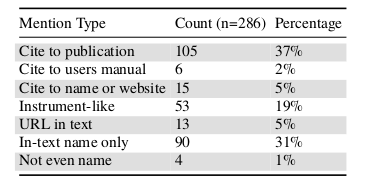
\includegraphics[scale=0.15]{aca2}
 \caption{Software citing in biology.\label{abb_2}}
\end{figure}

A lot of initiatives, being run by e.g., software companies, publishers, or
repositories have discussed and developed proprietary recommendations for
software citations. Mike Jackson has given in his blog \cite{Jackson} a
detailed state of the art analysis and pitfalls of software citation and
recommendations for a better citation practise. Currently, the FORCE 11
Software Citation Working group \cite{SoftwareCitationWG}, an international
initiative of more than 50 information experts from different scientific areas,
has discussed basic concepts for software citation. As one result the group has
published the Software Citation Principles (SCPs)
\cite{SoftwareCitationPrinciples}. They emphasize that software is a legitimate
product of research and therefore must be citable.  The six principles address
the importance of software within research which should manifest that all
relevant software will be cited, that software citations should facilitate
giving credit and attribution to the developers and contributors of software,
include methods for a unique identification, refer to persistent information
about software, should facilitate access to the software, and provide accurate
information about software (e.g., the version used). The SCPs define a general
frame for software citations and moreover formulate principles for maintaining
of information about software.

The SCPs do not discuss the realization of the principles.  This is planned to
be subject for a follow-up working group.

Exact information about software -- together with the data used -- is a
necessary condition to evaluate and reproduce scientific results which were
achieved by using mathematical software. Therefore, for the citation format,
the following recommendation is given: ``We recommend that all text citation
styles support the following: a) a label indicating that this is software,
e.g., [software], potentially with more information such as [Software: Source
  Code], [Software: Executable], or [Software: Container], and b) support for
version information, e.g., Version 1.8.7'' \cite{SoftwareCitationPrinciples}.
Each researcher who uses a software for research and publishes her or his
results (e.g., in form of a paper, software or data file) is recommended to
cite software according to this recommendation.

The mathematical community uses the {\TeX} format for publishing. References
are encoded in the (outdated) Bib{\TeX} format or, more up to date, in the
Bib{\LaTeX} format. Actually, neither Bib{\TeX} nor Bib{\LaTeX} support a type
``software''. Up to now, the Bib{\LaTeX} standard contains no special document
type for software. Software must be typed as ``misc''. A pragmatic
recommendation is that it should be added to the title if a citation refers to
a software, together with detailed information about the software instance.
This could be done in the following form: title [Software:special type (Source
  Code, Package, Executable, Library, Other)] [Version or release or URL and/or
  date of the update and /or date of the download]. This would be a first step
to a better software citation practice and provides the required information
for the human user.

A more rigorous and Semantic Web compatible solution would be an extension of
Bib{\LaTeX} standard. Bib{\LaTeX} together with the back-end software Biber
provides the opportunity to define new document types, e.g., software and the
corresponding fields.  A prototype for a {\TeX} implementation is under
development within the framework of the swMATH activities. It is planned to
provide a template for {\TeX} encoding of software citations.

The Bib{\LaTeX} encoding allows also a simple transformation to other formats,
e.g., JSON, which can be used for a machine-based semantic processing of
software citations.

Comment: Also software which cites another software should contain the
corresponding notations. This could be done by separate citation files which
are encoded in the same form as for papers, e.g., in Bib\LaTeX.

The SCPs recommend that ``the software itself should be cited on the same base
as any other research product'', and should have a unique and persistent
identifier, preferably a DOI. This does not mean that the DOI is assigned to
the software code. Outdated software is often removed from the Web. Instead,
``the software identifier should resolve to a persistent landing page that
contain metadata and a link to the software itself, rather than directly to the
source code files, repository, or executable'',
\cite{SoftwareCitationPrinciples}.  The problem of persistent identifiers and
landing pages, especially of a DOI, is connected with additional efforts. Up to
now, the existing landing pages, e.g., portals and software directories,
provide only metadata about families of software which is offered under the
same name, not about versions.

It seems to make sense that -- similar to publications -- persistent
identifiers should be provided and maintained by special information services
which integrate the information about software in a subject and make it
available.  The SCPs make clear that a citation standard would be very helpful
for better software information but it is only a building block in a better
digital information infrastructure for software and scientific information in
general. That is why we continue with a brief description about Web resources
which are relevant for mathematical software information.

\section{The landscape of mathematical software information in the Web}

The landscape of Web resources of mathematical software information is
heterogeneous, widely distributed, and has different layers.  Here is an
incomplete list of the relevant resources:
\begin{itemize}
\item{\textit{Individual websites of a software}}\\ This is in some sense the
  basic layer of the software information infrastructure. Websites exist for
  many though not all software packages (from our experiences in the swMATH
  project we estimate that nearly two thirds of mathematical software packages
  provide information on own websites). Typically, these websites contain a lot
  of detailed information about a software, documentation, manuals, tutorials,
  software code (if the software is free), the programming language used,
  contact information, usability and licences, hard- and software requirements,
  publication lists, etc.
\item{\textit{Repositories}}\\ Software repositories as ``The Comprehensive R
  Archive Network (CRAN)'' \cite{CRAN} or ``The Comprehensive Perl Archive
  Network (CPAN)'' \cite{CPAN} provide and maintain metadata plus the source
  code of software collections. CRAN is a repository for statistical software
  written in the R language and presents standardized meta information, the
  version history, and links to the source code for nearly 10,000 packages.
\item{\textit{Portals, directories and information services}}\\ Portals or
  directories of software provide lists of software, metadata, and
  links. ``Fachgruppe Computeralgebra'' \cite{FAG} or ``SIGSAM'' \cite{SIGSAM}
  offers structured webpages for computer algebra systems. These services, like
  the Symbolic Data project \cite{SD}, are not limited to information about
  software but also on conferences and workshops, researchers, and data. We
  will discuss this in more detail below.

An informative list of computer algebra systems can also be found in Wikipedia
\cite{WikipediaCAS}.

\begin{figure}[h]
  \centering
  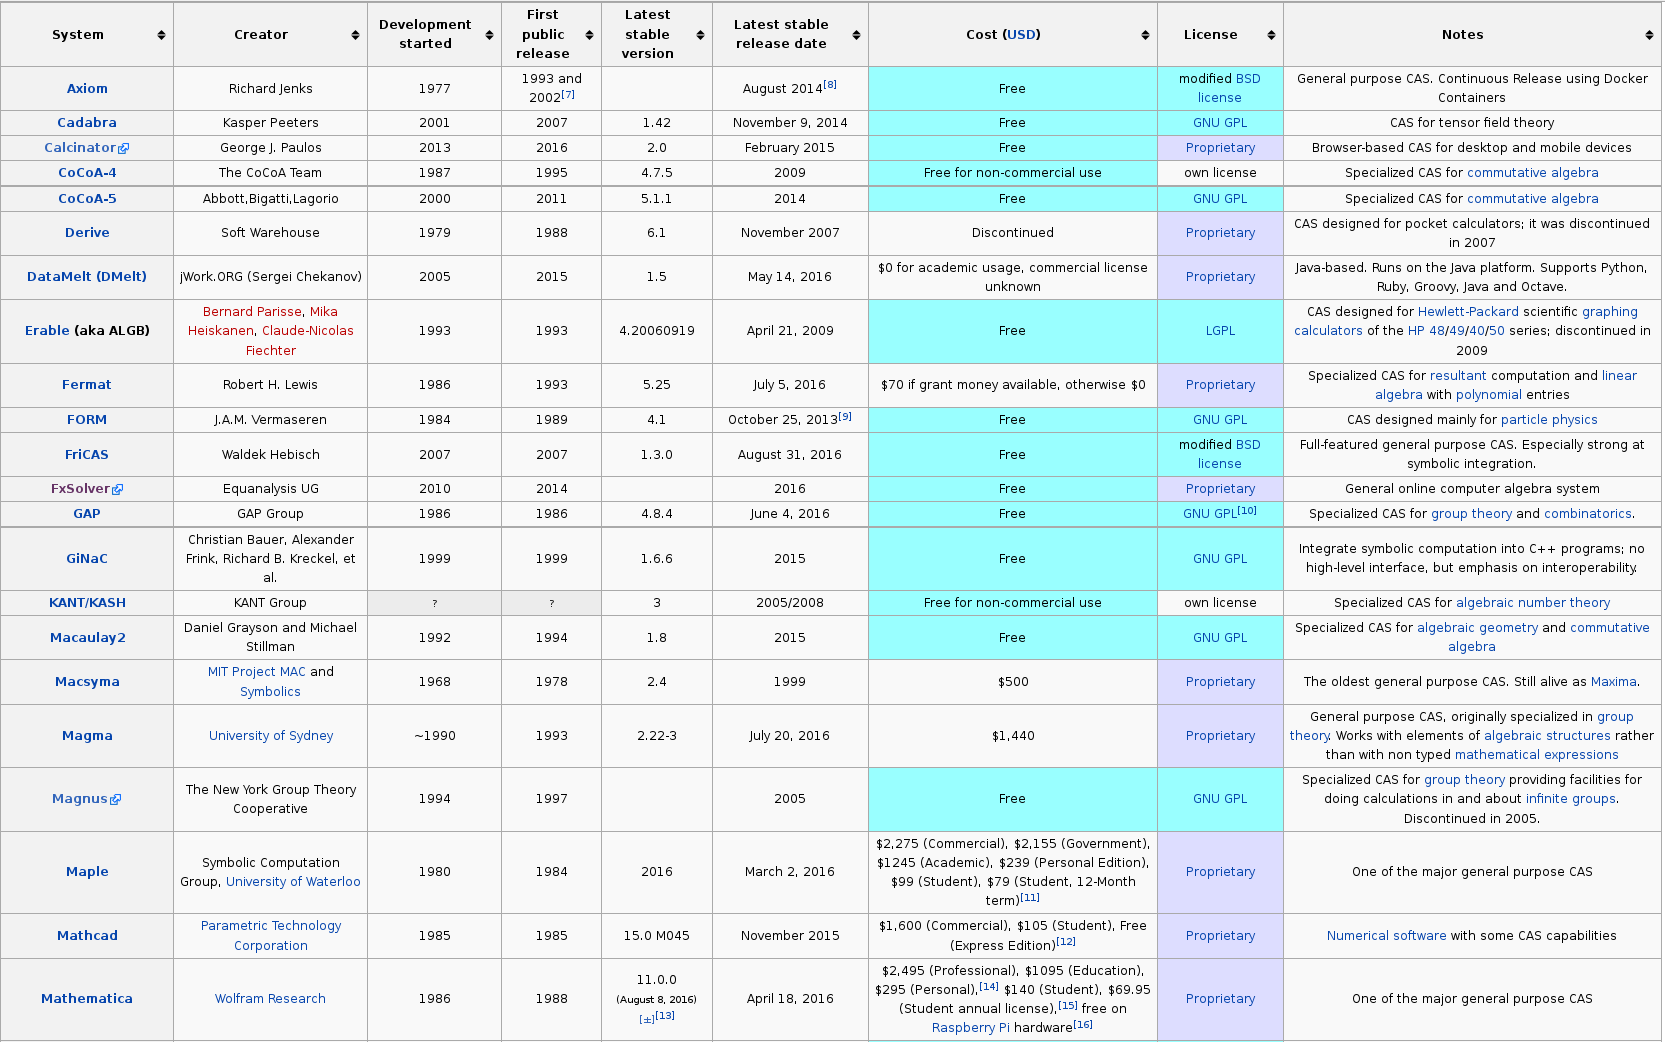
\includegraphics[scale=0.22]{aca3}
  \caption{A snippet of the Wikipedia (I): list of computer algebra
    systems.\label{abb_3}}
\end{figure}

\begin{figure}[h]
  \centering
  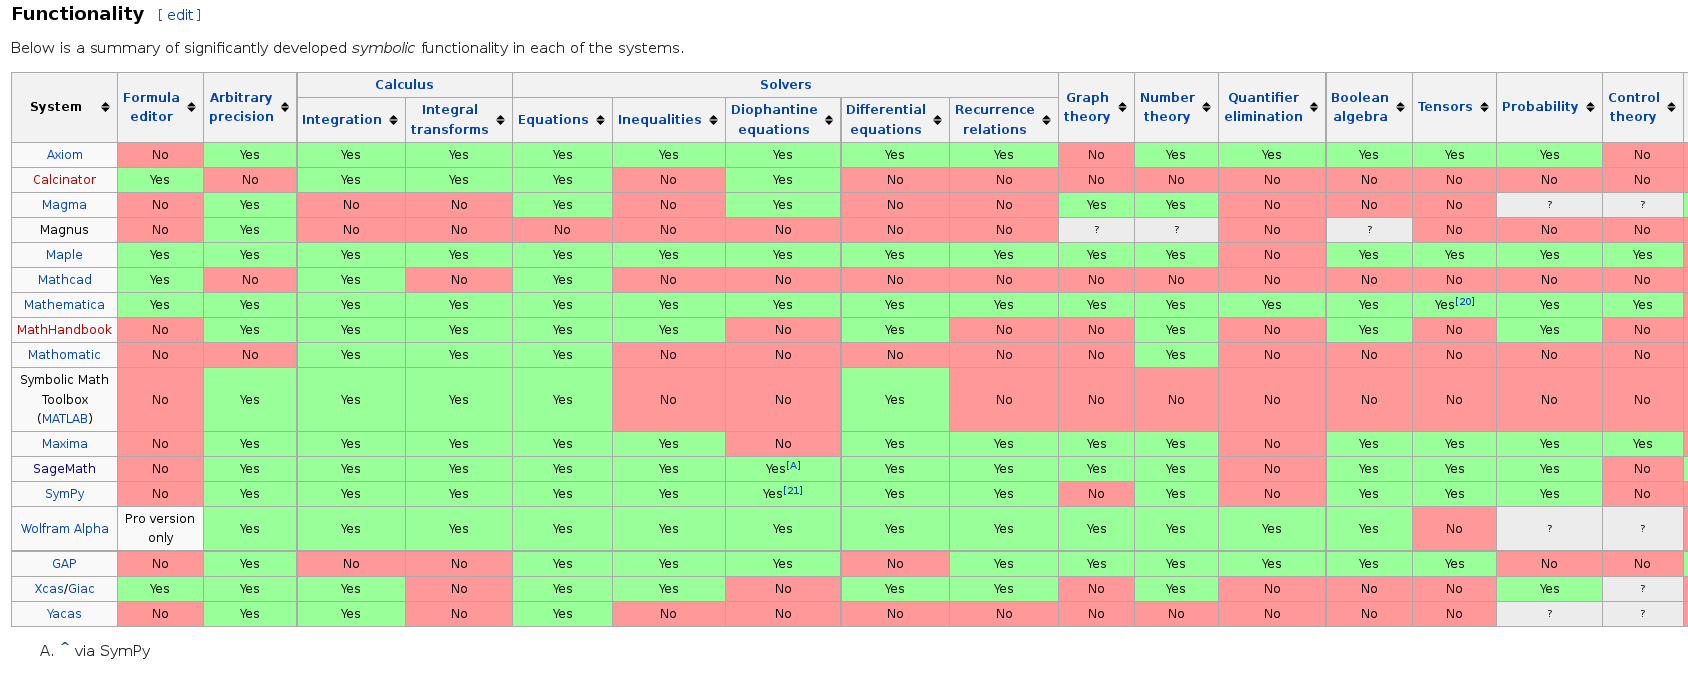
\includegraphics[scale=0.22]{aca4}
  \caption{A snippet of Wikipedia (II): functionalities of computer algebra
    systems \label{abb_4}}
\end{figure}

The lists mentioned here are manually maintained and updated, have different
structure also for metadata and are weakly coordinated, see also the remarks
about the Computer Algebra Social Network (CASN) below.
\item{\textit{Further resources}}\\
\begin{itemize}
\item{Services}\\ Software can be available in different forms, e.g., as a
  service (cloud computing, Class Group Database \cite{CCDb,MKD}).
\item{Journals specialized in mathematical software}\\ Also the software
  journals are mentioned here because they play a pioneering role for the
  quality control and evaluation of software. There exists a number of journals
  specialized in mathematical software, e.g., the Journal of Software for
  Algebra and Geometry \cite{JAG}, where the peer reviewing also includes
  mathematical software.
\item{Conferences (including proceedings) on CASs}
\end{itemize}
\end{itemize}
Moreover, mathematical software must be considered in its context which is
given by mathematical theories, algorithms, programming languages,
applications, data, e.g., benchmarks and data formats, and also the developers
and user communities of software. Context analysis is also an important method
to build up and develop powerful machine-based information services for
mathematical software which will be demonstrated by the swMATH concept in the
next section.\par

\section{swMATH}
\subsection{The publication-based-approach}
An important feature of the swMATH \cite{swMATH} concept, the publication-based
approach, has its origin in the analysis of context information. Instead of
analyzing mathematical publications for software citations and information
about software, the database zbMATH \cite{zbMATH} is used.  Especially, the
zbMATH database contains the following data of publications which are of
relevance for the analysis: title, keywords, reviews or abstracts, reference
lists, and classification codes.  The data analysis and knowledge generation of
the swMATH approach has several steps:
\begin{enumerate}
\item{\textit{Identification of software references within the zbMATH
    data}}\\ The title, the review or abstract, and the reference lists of
  publications are searched for indicators for software references by heuristic
  means. Such indicators can be artificial names in combination with
  characteristic words as software, module, package, etc.  Of course, the
  methods used are very simple but work surprisingly well. The acceptance of a
  software citation standard corresponding to the recommendations given above
  would make the heuristic methods obsolete and permit a secure and complete
  identification of software.
\item{\textit{Extraction of information about software}}\\ Reviews and
  abstracts of a mathematical publication contain most of all content
  information, especially a description of the problems investigated, the used
  methods, and results. \\ For software references it is useful to distinct
  between two classes of publications: The publications which describe a
  software (labeled as ``standard publications'') and publications which use a
  software for solving a problem (labeled as ``user publications''). Both types
  provide different information about a software and are processed in different
  ways. Some information directly enters into swMATH, e.g., keywords or MSC
  codes.
\item{\textit{Aggregation and ranking of information}}\\ Currently, swMATH has
  nearly 16,000 entries on software packages and other mathematical research
  data which contain more than 215,000 software citations in more than 130,000
  publications. In other words, there is often a great number of publications
  citing a software. This allows to weight the information by the corresponding
  number of the keyword frequencies which is done in the keyword cloud, to
  create an ``acceptance profile'' of the software (citation graph) by the
  number of annual publications citing a software.  It's also possible to give
  some information about related software based on the MSC classification
  codes. The number of publications citing a software could also be used as a
  measure for credit to the developers. Further features are possible, e.g.,
  the definition of an application profile of the software. All this can be
  done automatically by heuristic means.
\end{enumerate}

\subsection{The Web-based approach}
The publication-based method is a powerful tool but has
limitations. Publications do not cover technical details about the
implementation, the programming language, or the required hard- and software
environment of a software. Typically, this information is given in manuals and
documentations. Also other context information, e.g., test data and benchmarks
or programming languages, are important for reproducing the results of a
publication. As said above, this kind of information can often be found on
other resources on the Web.

Therefore swMATH tries to enrich the information about software by adding
information from the Web. At first, swMATH tries to find the website of a
software and links it if the search was successful.  We have started to develop
methods for analyzing the websites, see \cite{TPDL}. For this purpose the
Internet Archive \cite{IA} is used which provides also the data from a lot of
websites of mathematical software from the past.  Also the information of some
repositories is integrated in swMATH.  swMATH shows that the analysis of
different resources is a promising way to run and maintain useful and efficient
information services for mathematical software.\par


\subsection{swMATH in a nutshell}

swMATH lists more than 100 entries for CASs. A swMATH search for ``computer
algebra system'' shows a list of CASs
\begin{figure}[h]
  \centering 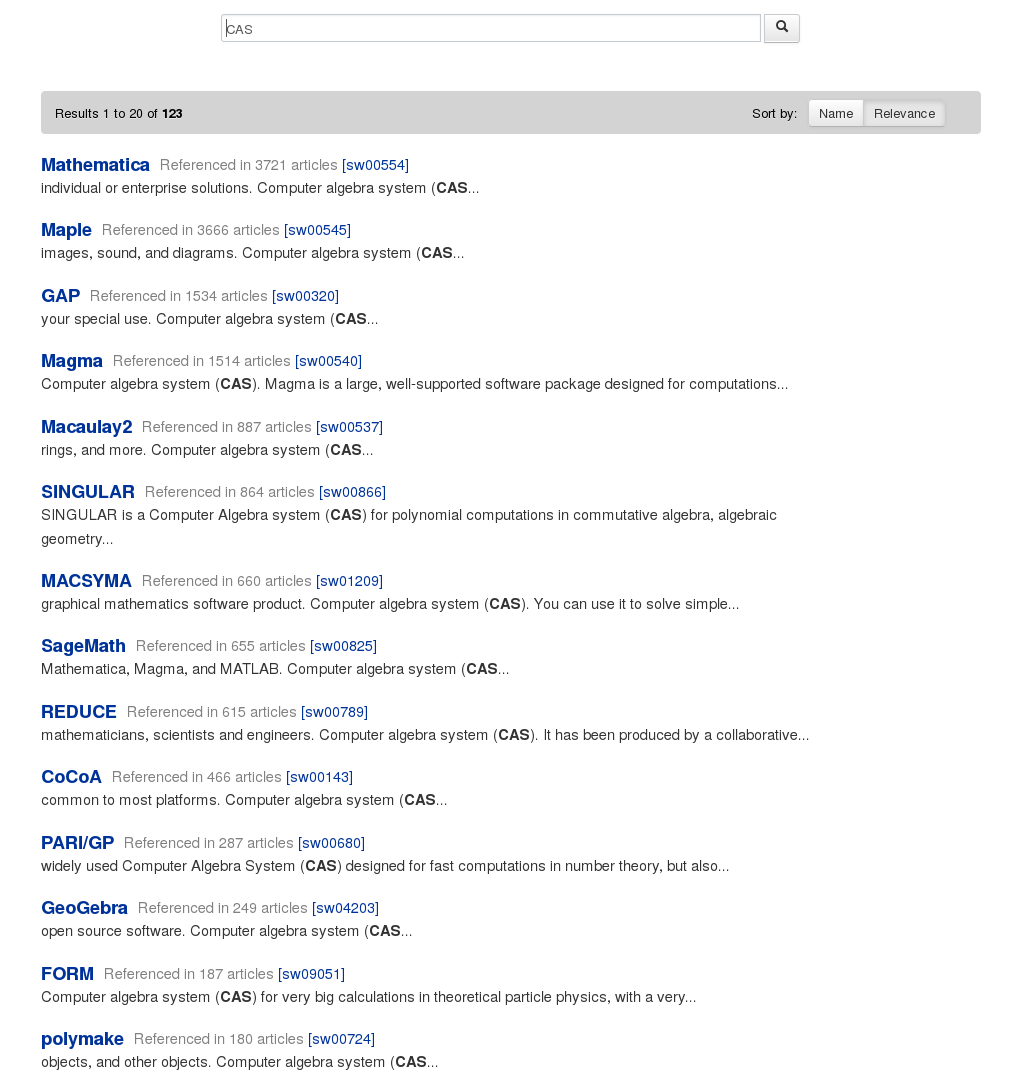
\includegraphics[scale=0.2]{aca5}
  \caption{A snippet of the swMATH list of computer algebra
    systems.\label{abb_5}}
\end{figure}

Each CAS is presented by an own webpage, see, e.g., a cutout of the swMATH
webpage for the software ``Singular'' in Fig. 6.
\begin{figure}[h]
  \centering
  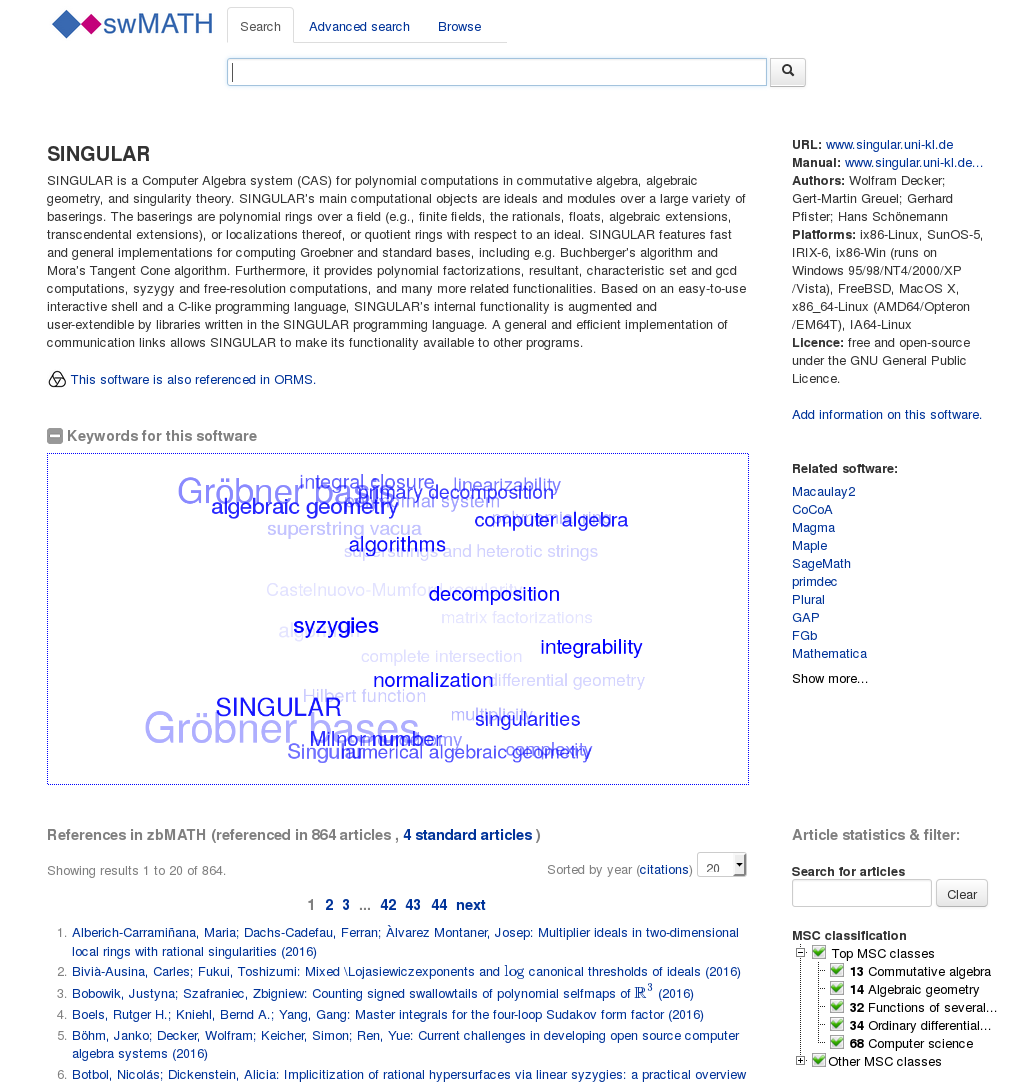
\includegraphics[scale=0.2]{aca6}
  \caption{A snippet of the swMATH webpage for the software
    ``Singular''.\label{abb_6}}
\end{figure}

Typically, swMATH provides the following information:
\begin{enumerate}
\item a list of mathematical software packages (and other related mathematical
  research data), as complete as possible
\item a persistent identifier (a five digit number) for each software,
\item metadata, especially about its content (description, keywords, MSC
  codes),
\item links  to the websites of the software (if existing).
\item a list of publications citing a software
\item a list of similar software
\item an acceptance profile for the software
\item links from the publications to the corresponding versions (currently only
  in the test version)
\item links to the Internet archive
\item links to manuals, documentation, source code, etc.
\end{enumerate}

Moreover, swMATH provides a simple and an extended search functionality.


\section{The Computer Algebra Social Network}
Software information is an important part of the scientific digital information
and communication infrastructure. The scientific digital infrastructure is
widely distributed and must be able to process and link heterogeneous
resources, e.g., information about researchers, publications, software,
conferences and workshop, etc. and data formats in a semantic way.  This
requires an active goal-oriented conceptual and technical cooperation between
different players. All relevant data must be digitized, semantically enriched
and encoded in a machine-understandable way.  The idea of the Computer Algebra
Social Network (CASN), for an overview on CASN see H.-G. Gr"abe \cite{CASN}, is
an advancement and continuation of the Symbolic Data concept. Established Web
technologies, especially RDF, should be used for the semantic annotation of
resources. Each resource, e.g., the servers of the German CA Fachgruppe or
SIGSAM, can become a node in this network. The RDF files of the metadata which
are created by the provider of a node guarantee that the information can be
automatically linked and is accessible via CASN. The swMATH service is
integrated in CASN.

\section{Summary and outlook -- what we can and should do}

A powerful and sustainable infrastructure for mathematical software information
is in the interest of developers and users.  It is also important for the
positioning and the role of this research subject in the sciences and in
society.  The infrastructure must be oriented towards the interests of the
developers and users. The mathematical community should actively take part and
influence the development.  Specifically, the information about software is
inconsistent, is distributed, not standardized, and not machine-processable,
which hampers the combination of heterogeneous resources of mathematical
software and related information. A better citation practice, standardization,
enrichment of the semantic information, coordination, and a better integration
of software as desired in the Open DreamKit project \cite{OpenDreamKit} opens
new perspectives for this research subject.  We need a broad dialogue and a
communication forum which brings the developers, the user communities,
information experts, and service providers together for a discussion of all
aspects. The symbolic computation community could play a pioneering role to
establish a sophisticated infrastructure for a mathematical subject which
covers all relevant resources. These include
\begin{itemize}
\item{definition of the overall goals and principles of an infrastructure for
  mathematical software}
\item{standardization}\\ for the authors: The authors should cite the software
  corresponding to the recommendations of the SCPs, especially marking up the
  type and give information about the versions, releases, etc,\\ for developers
  and service providers: There should be developed a standardized metadata
  scheme for mathematical software (analyzing the different facets of software
  information),\\ for service providers: The information should be provided in
  a machine-understandable way which supports a semantically sensible
  combination of information,\\ for service providers: Development of intuitive
  tools to support the standardized description of citations.
\item{a better linking of the information resources of software} for service
  providers: This requires a cooperation between the providers of the different
  services for software and its context and the development of user interfaces.
\end{itemize}

\section*{Acknowledgement}
We are grateful to the Fachgruppe Computeralgebra to help us reach a wider
audience by additionally publishing this article in the ``Computeralgebra
Rundbrief'', issue 60 (March 2017).

\bibliographystyle{plain}
\begin{thebibliography}{19}
\itemsep=0cm plus 0pt minus 0pt

\bibitem
%Label
{CCDb}
%Autoren
Boy, Maximilian:
%Titel
\newblock {A Database for Class Groups of Number Fields, homepage}.\\
%Zeitschrift
\newblock \url{http://www.mathematik.uni-kl.de/~numberfieldtables/}

\bibitem
%Label
{FAG}
%Autoren
Fachgruppe Computeralgebra:
%Titel
\newblock {Homepage}.\\
%Zeitschrift
\newblock \url{http://www.fachgruppe-computeralgebra.de/systeme/}

\bibitem
%Label
{swMATH}
%Autoren
FIZ Karlsruhe, ZIB Berlin:
%Titel
\newblock {swMATH Homepage}.
%Zeitschrift
\newblock \url{http://www.swMATH.org}

\bibitem
%Label
{zbMATH}
%Autoren
FIZ Karlsruhe:
%Titel
\newblock {zbMATH Homepage}.\\
%Zeitschrift
\newblock \url{http://www.zbMATH.org}

\bibitem
%Label
{Conferences}
%Autoren
Gr\"abe, Hans-Gert:
%Titel
\newblock {RDF File of CA Conferences}.\\
%Zeitschrift
\newblock \url{http://symbolicdata.org/rdf/Conferences/}


\bibitem
%Label
{SD}
%Autoren
Gr"abe, Hans-Gert:
%Titel
\newblock {The SymbolicData Project}.
%Zeitschrift
\newblock \url{http://wwww.symbolicdata.org}

\bibitem
%Label
{CASN}
%Autoren
Gr\"abe, Hans-Gert:
%Titel
\newblock {The SymbolicData Project -- Maturing the Computer Algebra Social
  Network Perspective}.
%Zeitschrift
\newblock {{\em Computeralgebra Rundbrief 59, p. 17-21},\\
\url{http://symbolicdata.org/Papers/aca-16-paper.pdf}}

\bibitem
%Label
{TPDL}
%Autoren
Holzmann, Helge; Sperber, Wolfram; Runnwerth, Mila:
%Titel
\newblock {Archiving Software Surrogates on the Web for Future Reference}.
%Zeitschrift
\newblock {\em In: Norbert Fuhr, L\'aszlo Kov\'acs, Thomas Risse, Wolfgang
  Neidl, Research and Advanced Technology for Digital Libraries: 20th
  International Conferences on Theory and Practice of Digital Libraries, TPDL
  2016, Hannover 2016, LNCS 9819, p. 215 - 226,}

\bibitem
% Label
{Howison&Bullard2015}
% Autoren
Howison, J.; Bullard, J.:
% Titel
\newblock{Software in the scientific literature: Problems with seeing, finding,
  and using software mentionend in the biology literature}.
% Zeitschrift
\newblock {\em Journal of the Association for Information Science and
  Technology, 2015,}\\ \url{http://dx.doi.org/10.1002/asi.23538}

\bibitem
%Label
{IA}
%Autoren
Internet Archive:
%Internet Archive
%Titel
\newblock {Homepage}.\\
%Zeitschrift
\newblock \url{https://archive.org/web/}


\bibitem
% Label
{Jackson}
% Autoren
Jackson, Mike:
% Titel
\newblock {How to cite and describe software?}\\
% Zeitschrift
\newblock \url{https://www.software.ac.uk/how-cite-and-describe-software}

\bibitem
%Label
{JAG}
%Autoren
Journal of Software for Algebra and Geometry Editorial Board:
%Titel
\newblock {Homepage}.\\
%Zeitschrift
\newblock \url{http://msp.org/jsag/about/cover/cover.html}

\bibitem
%Label
{MKD}
%Autoren
Kl\"uners, J; Malle, G:
%Titel
\newblock {A Database for Number Fields, homepage}.\\
%Zeitschrift
\newblock \url{http://galoisdb.math.uni-paderborn.de/}

\bibitem
%Label
{CPAN}
%Autoren
Perl Foundation:
%Titel
\newblock {The Comprehensive Perl Archive Network}.
%Zeitschrift
\newblock \url{http://www.cpan.org/}


\bibitem
%Label
{CRAN}
%Autoren
R Foundation:
%Titel
\newblock {The Comprehensive R Archive Network}.
%Zeitschrift
\newblock \url{https://cran.r-project.org/}

\bibitem
% Label
{SoftwareCitationPrinciples}
%%Autoren
Smith, Arfon M.; Katz, Daniel S.; Niemeyer, Kyle E.; FORCE11 Software Citation
Working Group:
%% Titel
\newblock {Software citation principles}.\\
%% Zeitschrift
\newblock{{\em Peer J. Computer Science 2:e86, 2016},\\
 \url{https://doi.org/10.7717/peerj-cs.86}}

\bibitem
%Label
{SIGSAM}
%Autoren
Special Interest Group on Symbolic and Algebraic Manipulation of the ACM:
%Titel
\newblock {Homepage}.
%Zeitschrift
\newblock \url{http://www.sigsam.org/Resources/Software.html}


\bibitem
% Label
{SoftwareCitationWG}
%Autoren
Software Citation Working Group:
% Titel
\newblock {Homepage},
% Zeitschrift
\newblock \url{https://www.force11.org/group/software-citation-working-group}.

\bibitem
%Label
{OpenDreamKit}
%Autoren
Thi\'ery, Nicolas M.:
%Titel
\newblock {OpenDreamKit: Open Digital Research Environment Toolkit for the
  Advancement of Mathematics}.
%Zeitschrift
\newblock {{\em Computeralgebra Rundbrief 57, p. 17-18,}\\
\url{http://www.fachgruppe-computeralgebra.de/data/CA-Rundbrief/car57.pdf}}


\bibitem
%Label
{WikipediaCAS}
%Autoren
Wikipedia Community:
%Titel
\newblock {The Wikipedia Web page of CASs}.\\
%Zeitschrift
\newblock \url{https://en.wikipedia.org/wiki/Listofcomputeralgebrasystems}



\end{thebibliography}

%%%%%%%%%%%%%%%%%%%%%%%%%%%%%%%%%%%%%%%%%%%%%%%%%%%%%%%%%%%%%%%%%%%%%%%%%%%%%%%%

\end{document}
